\documentclass[12pt,a4paper]{article}
\usepackage[utf8]{inputenc}
\usepackage[ngerman]{babel}
\usepackage{amsmath}
\usepackage{amsfonts}
\usepackage{amssymb}
\usepackage{listings}
\usepackage{longtable}
\usepackage{tikz}

\usetikzlibrary{positioning}
%\usepackage{program}

%\usepackage{xcolor}%für die Farben

\usepackage{graphicx}
\graphicspath{ {./Graphik/} }


\usepackage{tikz}
\usetikzlibrary{shapes, snakes}

\title{Data Mining}
\author{Vincent Dahmen 6689845 \and Rafael Heid 6704828}


\begin{document}

\maketitle{}


\section*{1}
Der folgende Python Code zeigt die einzelnen Lösungen:

\lstinputlisting[language=Python]{Skript/4.1.py}

\section*{2}
\begin{enumerate}

	\item das gezeichnete Perzeptron
	\begin{figure}[h]
		\centering
		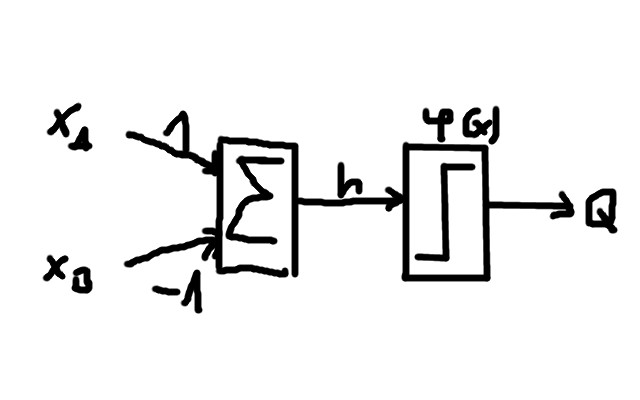
\includegraphics[scale=0.5]{AandNotB.jpg}
	\end{figure}
	%		\tikzset{basic/.style={draw,fill=blue!20,text width=1em,text badly centered}}
		\tikzset{input/.style={basic,circle}}
		\tikzset{weights/.style={basic,rectangle}}
		\tikzset{functions/.style={basic,circle,fill=blue!10}}
		
		\begin{tikzpicture}
		    \node[functions] (center) {};
		    \node[below of=center,font=\scriptsize,text width=4em] {Activation function};
		    \draw[thick] (0.5em,0.5em) -- (0,0.5em) -- (0,-0.5em) -- (-0.5em,-0.5em);
		    \draw (0em,0.75em) -- (0em,-0.75em);
		    \draw (0.75em,0em) -- (-0.75em,0em);
		    \node[right of=center] (right) {};
		        \path[draw,->] (center) -- (right);
		    \node[functions,left=3em of center] (left) {$\sum$};
		        \path[draw,->] (left) -- (center);
		    \node[weights,left=3em of left] (2) {$w_2$} -- (2) node[input,left of=2] (l2) {$x_2$};
		        \path[draw,->] (l2) -- (2);
		        \path[draw,->] (2) -- (left);
		    \node[below of=2] (dots) {$\vdots$} -- (dots) node[left of=dots] (ldots) {$\vdots$};
		    \node[weights,below of=dots] (n) {$w_n$} -- (n) node[input,left of=n] (ln) {$x_n$};
		        \path[draw,->] (ln) -- (n);
		        \path[draw,->] (n) -- (left);
		    \node[weights,above of=2] (1) {$w_1$} -- (1) node[input,left of=1] (l1) {$x_1$};
		        \path[draw,->] (l1) -- (1);
		        \path[draw,->] (1) -- (left);
		    \node[weights,above of=1] (0) {$w_0$} -- (0) node[input,left of=0] (l0) {$1$};
		        \path[draw,->] (l0) -- (0);
		        \path[draw,->] (0) -- (left);
		    \node[below of=ln,font=\scriptsize] {inputs};
		    \node[below of=n,font=\scriptsize] {weights};
		\end{tikzpicture}


	\item der Term 'linear separable' oder zu deutsch lineare Klassifierbarkeit gibt an, dass es eine lineare Funktion gibt, welche die Ergebnisse eideutig in 2 Klassen trennt (z.B. true - false)
		Bei der einfache boolschen Funktion AND ist dies tikz-graphik4.2.2, also im 2D Raum möglich, während es bei der Funktion XOR tikz-graphik4.2.3 nur im 3D Raum funktioniert.

	\item das kommentierte Programm
	\lstinputlisting{Skript/4.2.d.py}
\end{enumerate}

\section*{3}
\begin{itemize}
	\item 	Von 'overfitting' spricht man wenn ein neuronales Netz zu stark an einem Datensatz trainiert wird.
		Dies führt dazu, dass nur noch sehr ähnliche Daten richtig klassifiziert werden können

	\item 	'generalization' bezeichnet die Eigenschaft eines gut trainierten Netzes, möglichst allgemein Daten korrekt zu klassifizieren

	\item 	Um ein neuronales Netz zu trainieren werden mehrere Schritte durchlaufen:
		\begin{itemize}
			\item Das Netz such nach Gemeinsamkeinten im trainings-set
			\item alle gefundenen Regeln müssen auch im validation-set gelten
			\item Im test-set sieht man schließlich die Qualität der gefunden Regeln
		\end{itemize}
		Anschließend können die Parameter modifiziert werden bis die Qualität ausreichend ist

	\item 	Um ein overfitting zu vermeiden müssen die sets disjunkt sein
		Im Beispiel wird die Hälfte der Daten als traings-set und die verbleibenden 2 viertel als test- und validation set benutzt.

	\item 	Solange wie das Testset disjunkt mit dem Trainigsdaten ist, ist dies ausreichend.
	 	In der Praxis lässt man mehrere Traings- und Testzyklen laufen und verwendet dabeit verschiedene Partionen der Daten (dabei sind traings- und test-set jedoch stests disjunkt!)

\end{itemize}

\end{document}

